% TEX compiler = luatex
% copyright arturo salinas-aguayo 2025
\documentclass[12pt]{article}

\usepackage{graphicx}
\usepackage{amsmath}
\usepackage{array}
\usepackage{amsfonts}
\usepackage{fancyhdr}
\usepackage{geometry}
\usepackage{circuitikz}
\usepackage{subfigure}
\usepackage{caption}
\usepackage{karnaugh-map}
\usepackage{bm}
\usepackage{float}

\geometry{letterpaper, margin=1in}
\graphicspath{ {../../images/} }

% Header and Footer
\pagestyle{fancy}
\fancyhf{}
\fancyhead[L]{ECE 2001 - Lab 04: Generating and Measuring Sinusoidal Signals: A Sound System}
\fancyhead[R]{\thepage}
\setlength{\headheight}{15pt}

\author{Arturo Salinas-Aguayo}
\title{Lab 04: Generating and Measuring Sinusoidal Signals: A Sound System}
% theorem set
\newtheorem{example}{Example}
% Example block environment
\newenvironment{examp}
{\vspace{0.5cm}
 \hrule
\vspace{0.5cm}
\begin{example}}
{\hrule
\vspace{0.5cm}
\end{example}}

\begin{document}
\newcommand{\closure}[2][3]{%
	{}\mkern#1mu\overline{\mkern-#1mu#2}}
\newcommand\ncoverline[1]{\mkern1mu\overline{\mkern-1mu#1\mkern-1mu}\mkern1mu}
% Title Page
\begin{titlepage}
	\centering
	\vspace*{3cm}
	\huge\textbf{Lab 04: Generating and Measuring Sinusoidal Signals: A Sound System}\\
	\vspace{5cm}
	\Large\textbf{Arturo Salinas-Aguayo}\\
	\normalsize
	ECE 2001 Electrical Circuits\\
	Dr. David J. Giblin, Section 331.660.701.810-1253\\
	Mechanical Engineering Department
	\vfill
	
\includegraphics[scale=0.1]{uconnlogo}\\
	College of Engineering, University of Connecticut\\
	\scriptsize{Coded in \LaTeX}
	\vspace*{1cm}
\end{titlepage}
\tableofcontents
\newpage
\section{Abstract}
Building off from the introduction of the Operational Amplifier, this weeks
experimental work introduces a practical perspective on the utilization of the
chip: An Audio Amplifier. High quality audio systems are almost synonymous with
high quality electrical engineering design, which is to say that designing and
creating an electrical system which can take a signal and amplify it through
several stages and produce an output which is not distorted, but also clear
enough to be understood and interpreted on a wide spectrum of uses is
difficult. This experiment work introduces a simple way to accomplish this
through the use of rudimentary speakers and microphones, as well as the
operational amplifier circuit. It also serves as an introduction to utilizing
oscilloscopes for signal analysis and troubleshooting.
\newpage
\section{Introduction}
The heartbeat of a discrete signal is its ability to be interpreted through
different domains of which the time domain is the most easily understood by
humans. The human interprets time well and is able to define lengths of data
quite well in this domain, for example how long a piece of music lasts, or a
film on the big screen. We measure and base our experiences off this, and with
rudimentary time measuring devices some of the most important discoveries in
science have been made, propelling us to the modern understanding of the world
around use today.

In order to interpret these signals in an electrical circuit, oscilloscopes have
been developed to be able to display waveforms depending on the target signals
we wish to obtain. Varying signals such as an AC voltage, a response to a
digital circuit, or the multiplexed analog signal of hundreds of signals can be
read and interpreted using these scopes which allow for the further
troubleshooting of electrical circuits.

This experimental work starts out straight forward with realizing what has only
been seen in schematics thus far, the ideal current source, which on paper
supplies a constant current without changing other physical values of the
circuit. In order to achieve this, two abstract switches in the form of P-Type
and N-Type MOSFETs are utilized in conjunction with an operational amplifier at
the output in order to create a circuit called a "push-pull" amplifier.
The details of the MOSFET are kept ambiguous at this stage, and thus will not be
covered in this report. The other sections of the experiment however has a
rudimentary audio amplifier get realized which can be used as a loud speaker.
\section{Theory}
\subsection{The Signal Generator}
The ADALM2000 device has many applications, several of which have been explored
in this experimental work. One of its key features is the signal generator,
which allows for the creation of various waveforms. In this experiment, a
mixture of signals is generated, specifically the sine wave, square wave, and
triangle wave. These waveforms serve distinct purposes in electronics and signal
processing, and their characteristics significantly influence the behavior of
connected circuits.

\subsubsection{The Sine Wave}
A sine wave is a smooth, continuous waveform that represents a pure frequency
with no harmonics. Mathematically, it is described by the function:

\begin{equation} v(t) = A \sin(2\pi f t + \phi) \end{equation}

where \( A \) is the amplitude, \( f \) is the frequency in hertz, \( t \) is
time, and \( \phi \) is the phase shift. Sine waves are fundamental in audio
signal processing, telecommunications, and AC circuit analysis.

In this experiment, sine waves are used to test audio equipment, specifically an
electret condenser microphone and an 8W speaker. The smooth nature of the
waveform ensures that only a single frequency component is being tested at a
time, making it ideal for assessing the frequency response of the system.

\subsubsection{The Square Wave} A square wave is a non-sinusoidal waveform that
alternates between two distinct voltage levels with instantaneous transitions.
It is mathematically represented as:

\begin{equation} v(t) = \begin{cases} A,  & 0 \leq t < \frac{1}{2f}           \\
              -A, & \frac{1}{2f} \leq t < \frac{1}{f}\end{cases} \end{equation}

where \( A \) is the peak amplitude and \( f \) is the frequency. Square waves
contain a fundamental frequency and an infinite series of odd harmonics, making
them useful for testing frequency response and transient behavior in circuits.

\subsubsection{The Triangle Wave} A triangle wave is a periodic waveform that
linearly ramps up and down between a maximum and minimum amplitude. It is
described by:

\begin{equation} v(t) = \begin{cases} \frac{4A}{T}t - A, & 0 \leq t <
              \frac{T}{2}                     \\ -\frac{4A}{T}t + 3A, & \frac{T}{2} \leq t < T\end{cases}
\end{equation}

where \( A \) is the peak amplitude and \( T \) is the period. Unlike square
waves, triangle waves contain fewer high-frequency harmonics, making them
suitable for testing linearity in audio applications.

\subsection{The Electret Condenser Microphone} An electret condenser
microphone is a type of microphone that uses a permanently charged dielectric
material (electret) to generate an electrical signal in response to sound
waves. It consists of a diaphragm, a backplate, and a built-in Field-Effect
Transistor (FET) for impedance matching.

When sound waves strike the diaphragm, it moves relative to the backplate,
causing a variation in capacitance. This change is converted into a voltage
signal that can be further amplified and processed. The microphone typically
requires an external bias voltage, often supplied through a resistor.

In this experiment, the electret condenser microphone is used to capture the
generated signals and convert them into electrical waveforms. Its response to
speech signals is analyzed and used in the calculation to create an amplifier
suitable for the speaker.

\subsection{The 8W Speaker}
The 8W speaker is an electroacoustic transducer
that converts electrical signals into sound waves. It operates on the
principle of electromagnetic induction, where an alternating current passing
through the voice coil creates a magnetic field that interacts with a
permanent magnet. This interaction causes the diaphragm to move, producing
audible sound.

The speaker’s performance is characterized by: \begin{itemize} \item
	      \textbf{Frequency Response:} The range of frequencies the speaker can
	      effectively reproduce.
	\item \textbf{Impedance:} The electrical resistance
	      the speaker presents to the driving circuit, typically measured in ohms.
	\item \textbf{Power Handling:} The maximum electrical power the speaker can
	      handle without distortion or damage. \end{itemize}

In this experiment, the speaker is driven by the ADALM2000’s signal generator to
analyze its ability to reproduce different waveforms. The interaction between
input waveforms and the speaker's mechanical response is observed to assess
proper amplification stage levels.

\subsection{The Summing Amplifier}
A summing amplifier is an operational
amplifier (op-amp) configuration that outputs the weighted sum of multiple input
signals. It follows the equation:

\begin{equation} V_{out} = -\left(\frac{R_f}{R_1} V_1 + \frac{R_f}{R_2} V_2 +
	\dots + \frac{R_f}{R_n} V_n\right) \end{equation}

where \( R_f \) is the feedback resistor, \( R_1, R_2, \dots, R_n \) are input
resistors, and \( V_1, V_2, \dots, V_n \) are input voltages.

Summing amplifiers are widely used in audio mixing, signal processing, and
control systems. They allow multiple signals to be combined into a single output
while maintaining proportional relationships.
\section{Experimental Procedures}
\subsection{Oscilloscopes and Signals}
To begin, the utilization of Scopy software alongside the ADALM2000 is
introduced by generating signals and displaying them as read by the hardware.

The specific wiring is gone over in detail to differentiate between the signal
generation leads and the oscilloscope leads. The ADALM2000 provides two signal
generator channels and two channels to read using the oscilloscope function
within Scopy.
\begin{enumerate}
	\item A 2kHz Sine Wave is generated with a Peak-to-Peak value of 4V and a DC
	      offset of 2V. See Figure \ref{fig:sinewave} for the Oscilloscope output.
	      \begin{figure}[H]
		      \centering
		      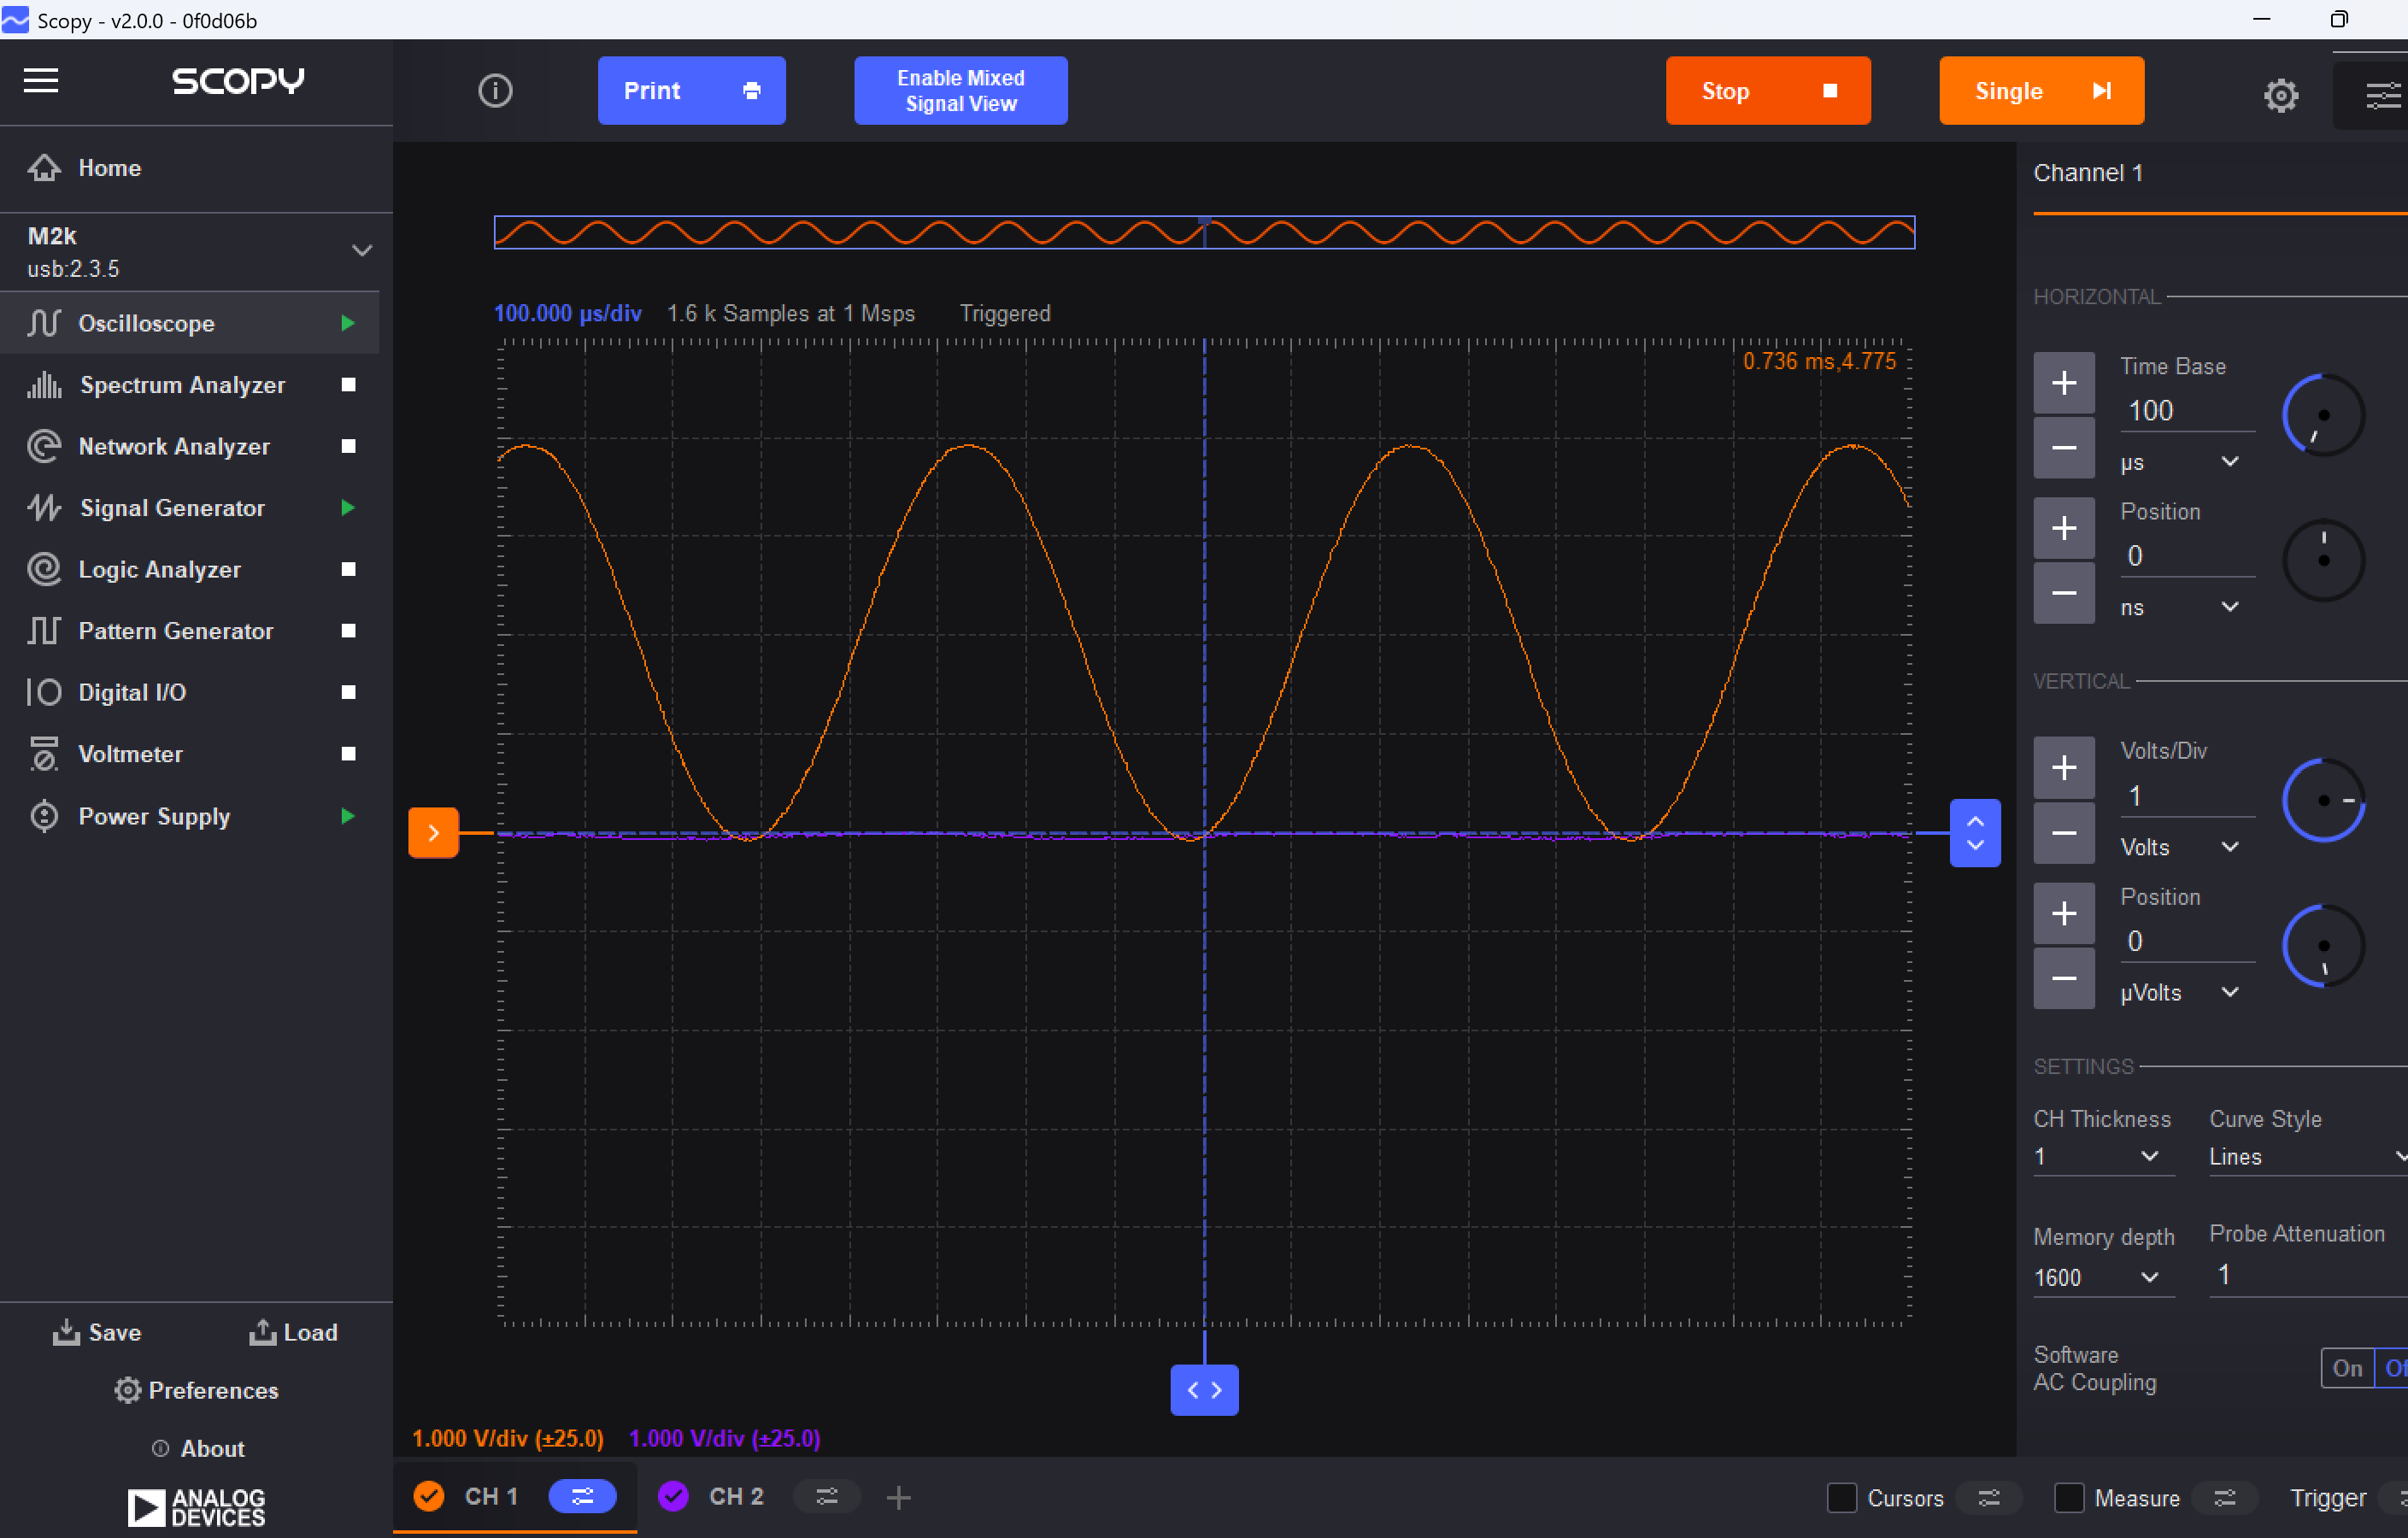
\includegraphics[width=14cm]{04_01}
		      \caption{A Sine Wave Output}
		      \label{fig:sinewave}
	      \end{figure}

	\item A 2kHz Square Wave is generated with the same Peak-to-Peak values of 4V
	      and a 2V DC Offset. Noise is introduced and gets interpreted by subtle quivers
	      in the square wave signal as shown in Figure \ref{fig:squarewave}

	      \begin{figure}[H]
		      \centering
		      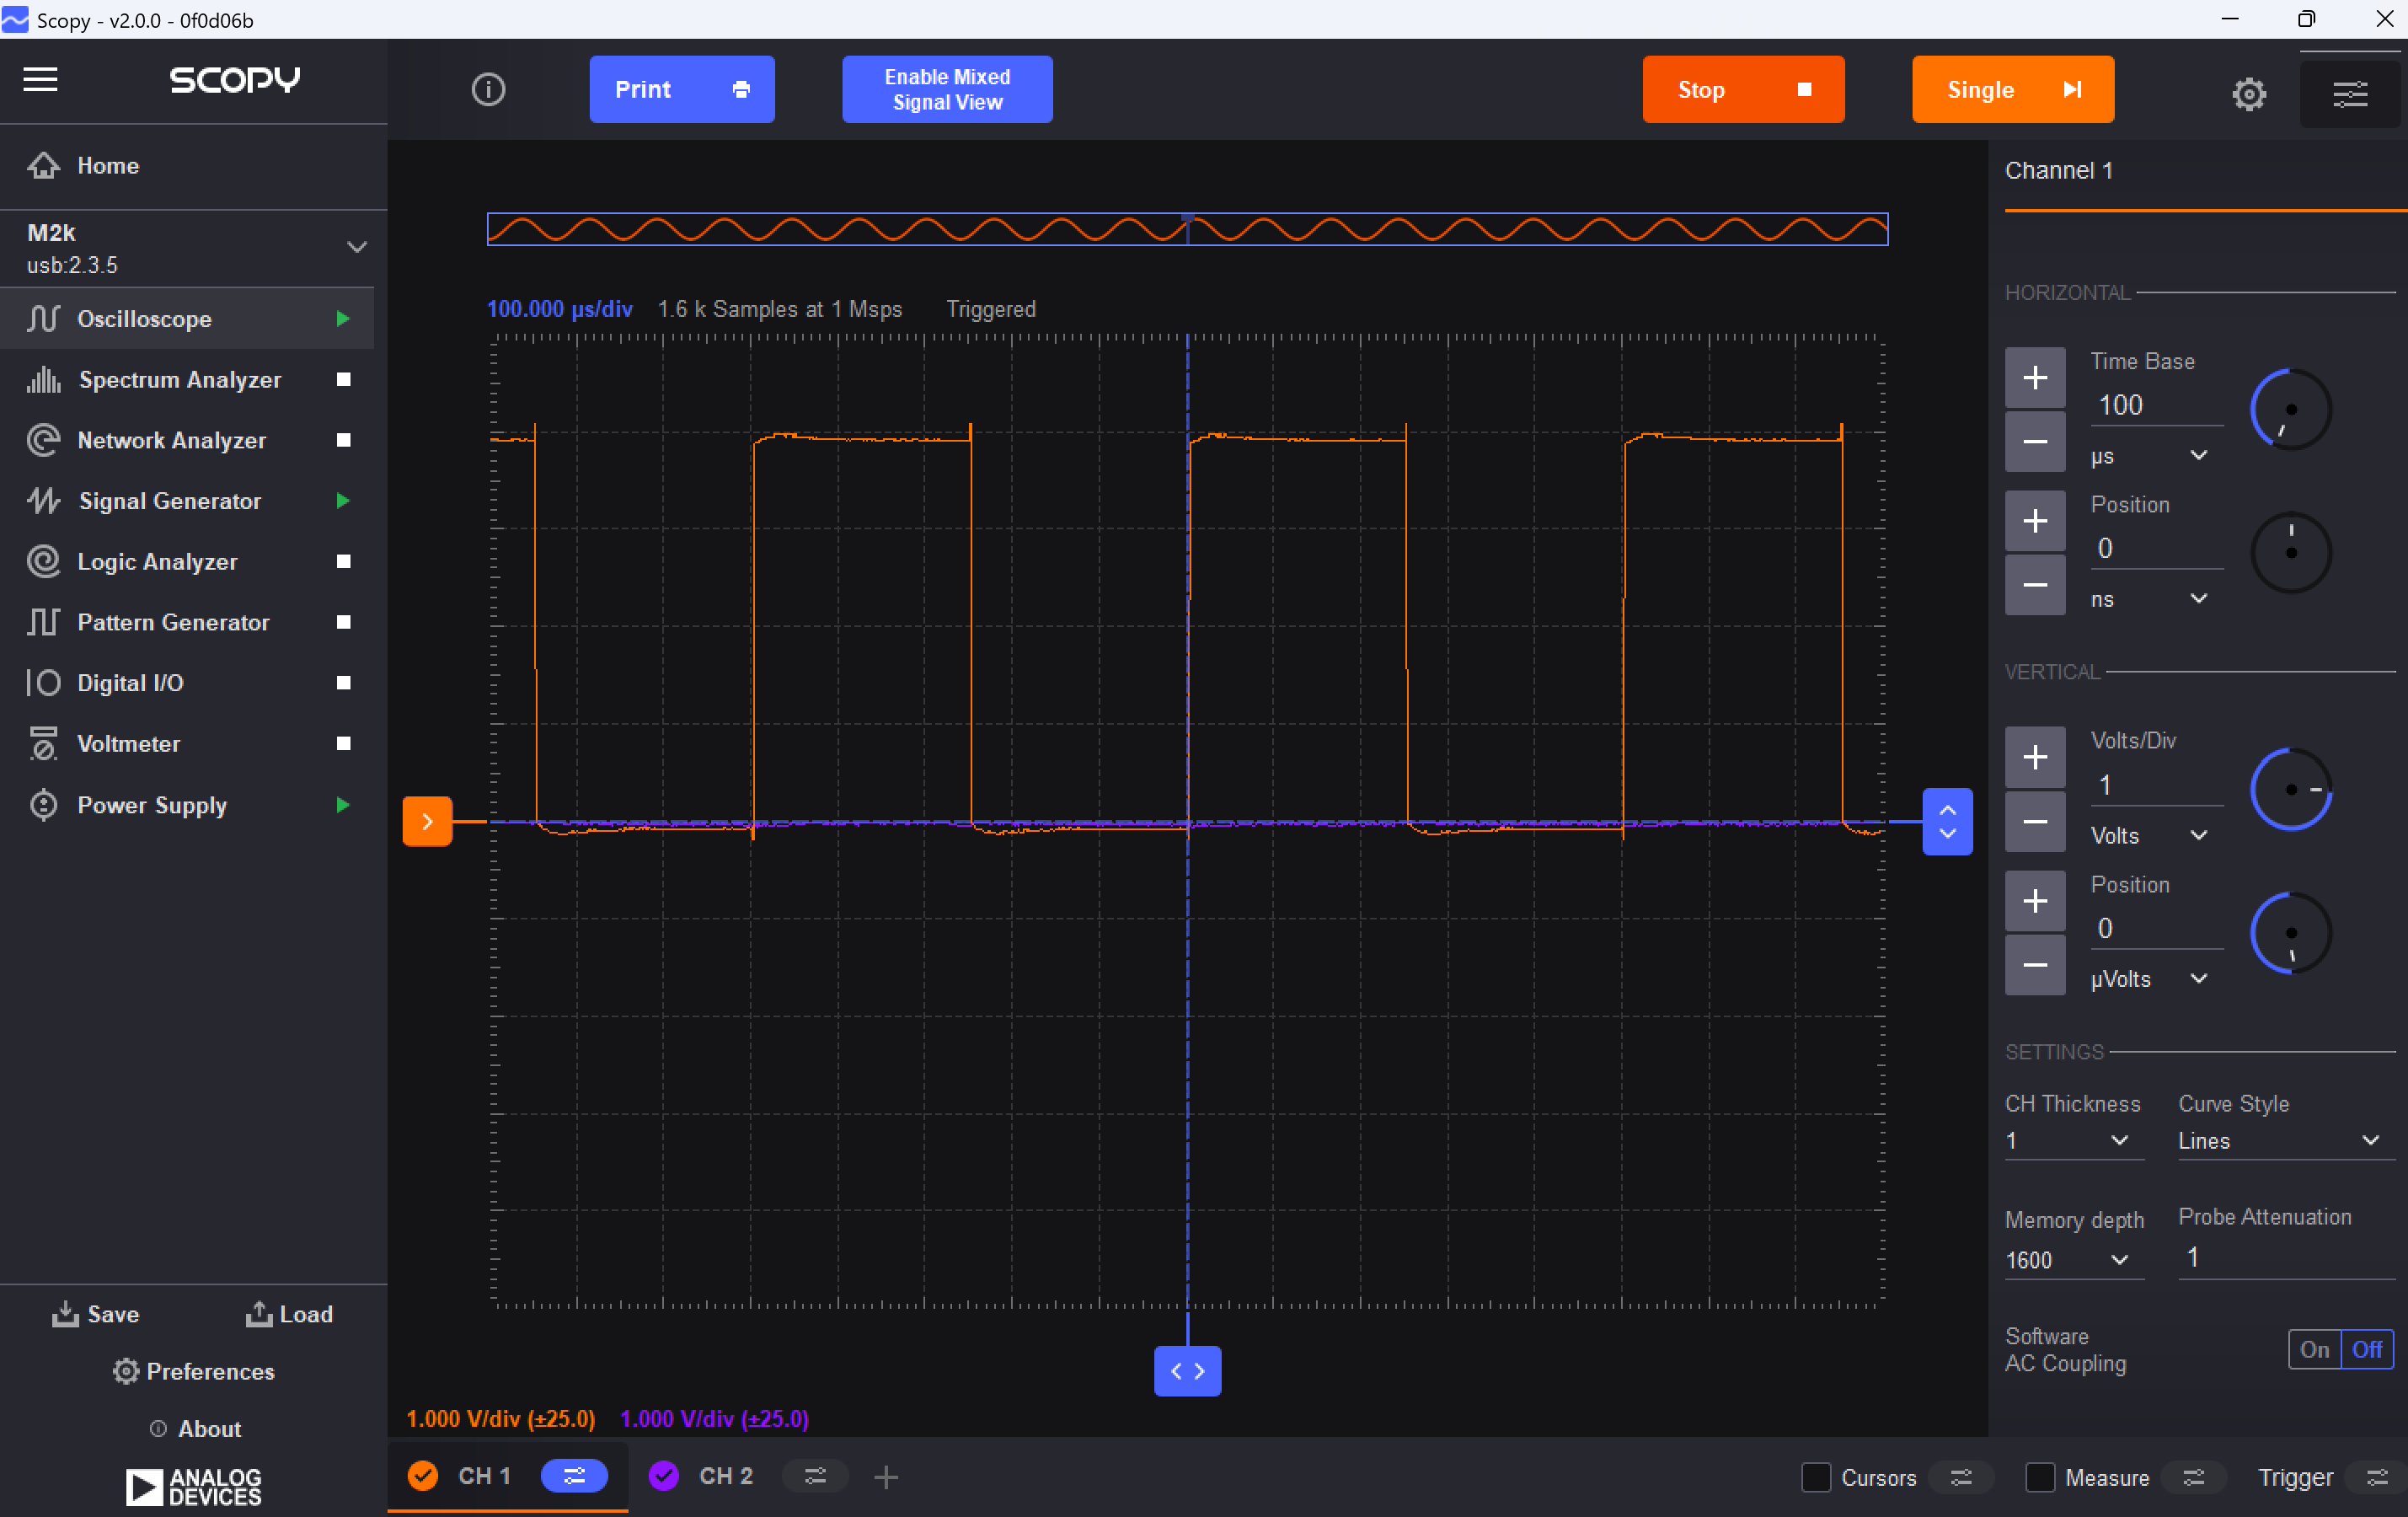
\includegraphics[width=14cm]{04_02}
		      \caption{A Square Wave Output}
		      \label{fig:squarewave}
	      \end{figure}

	\item Finally, a 2kHz Triangle Wave is generated with the same values. This
	      provided a challenge in utilizing the oscilloscope trigger as the signal was
	      quite dirty, nevertheless it was able to be displayed in crisp resolution as
	      in Figure \ref{fig:trianglewave}


	      \begin{figure}[H]
		      \centering
		      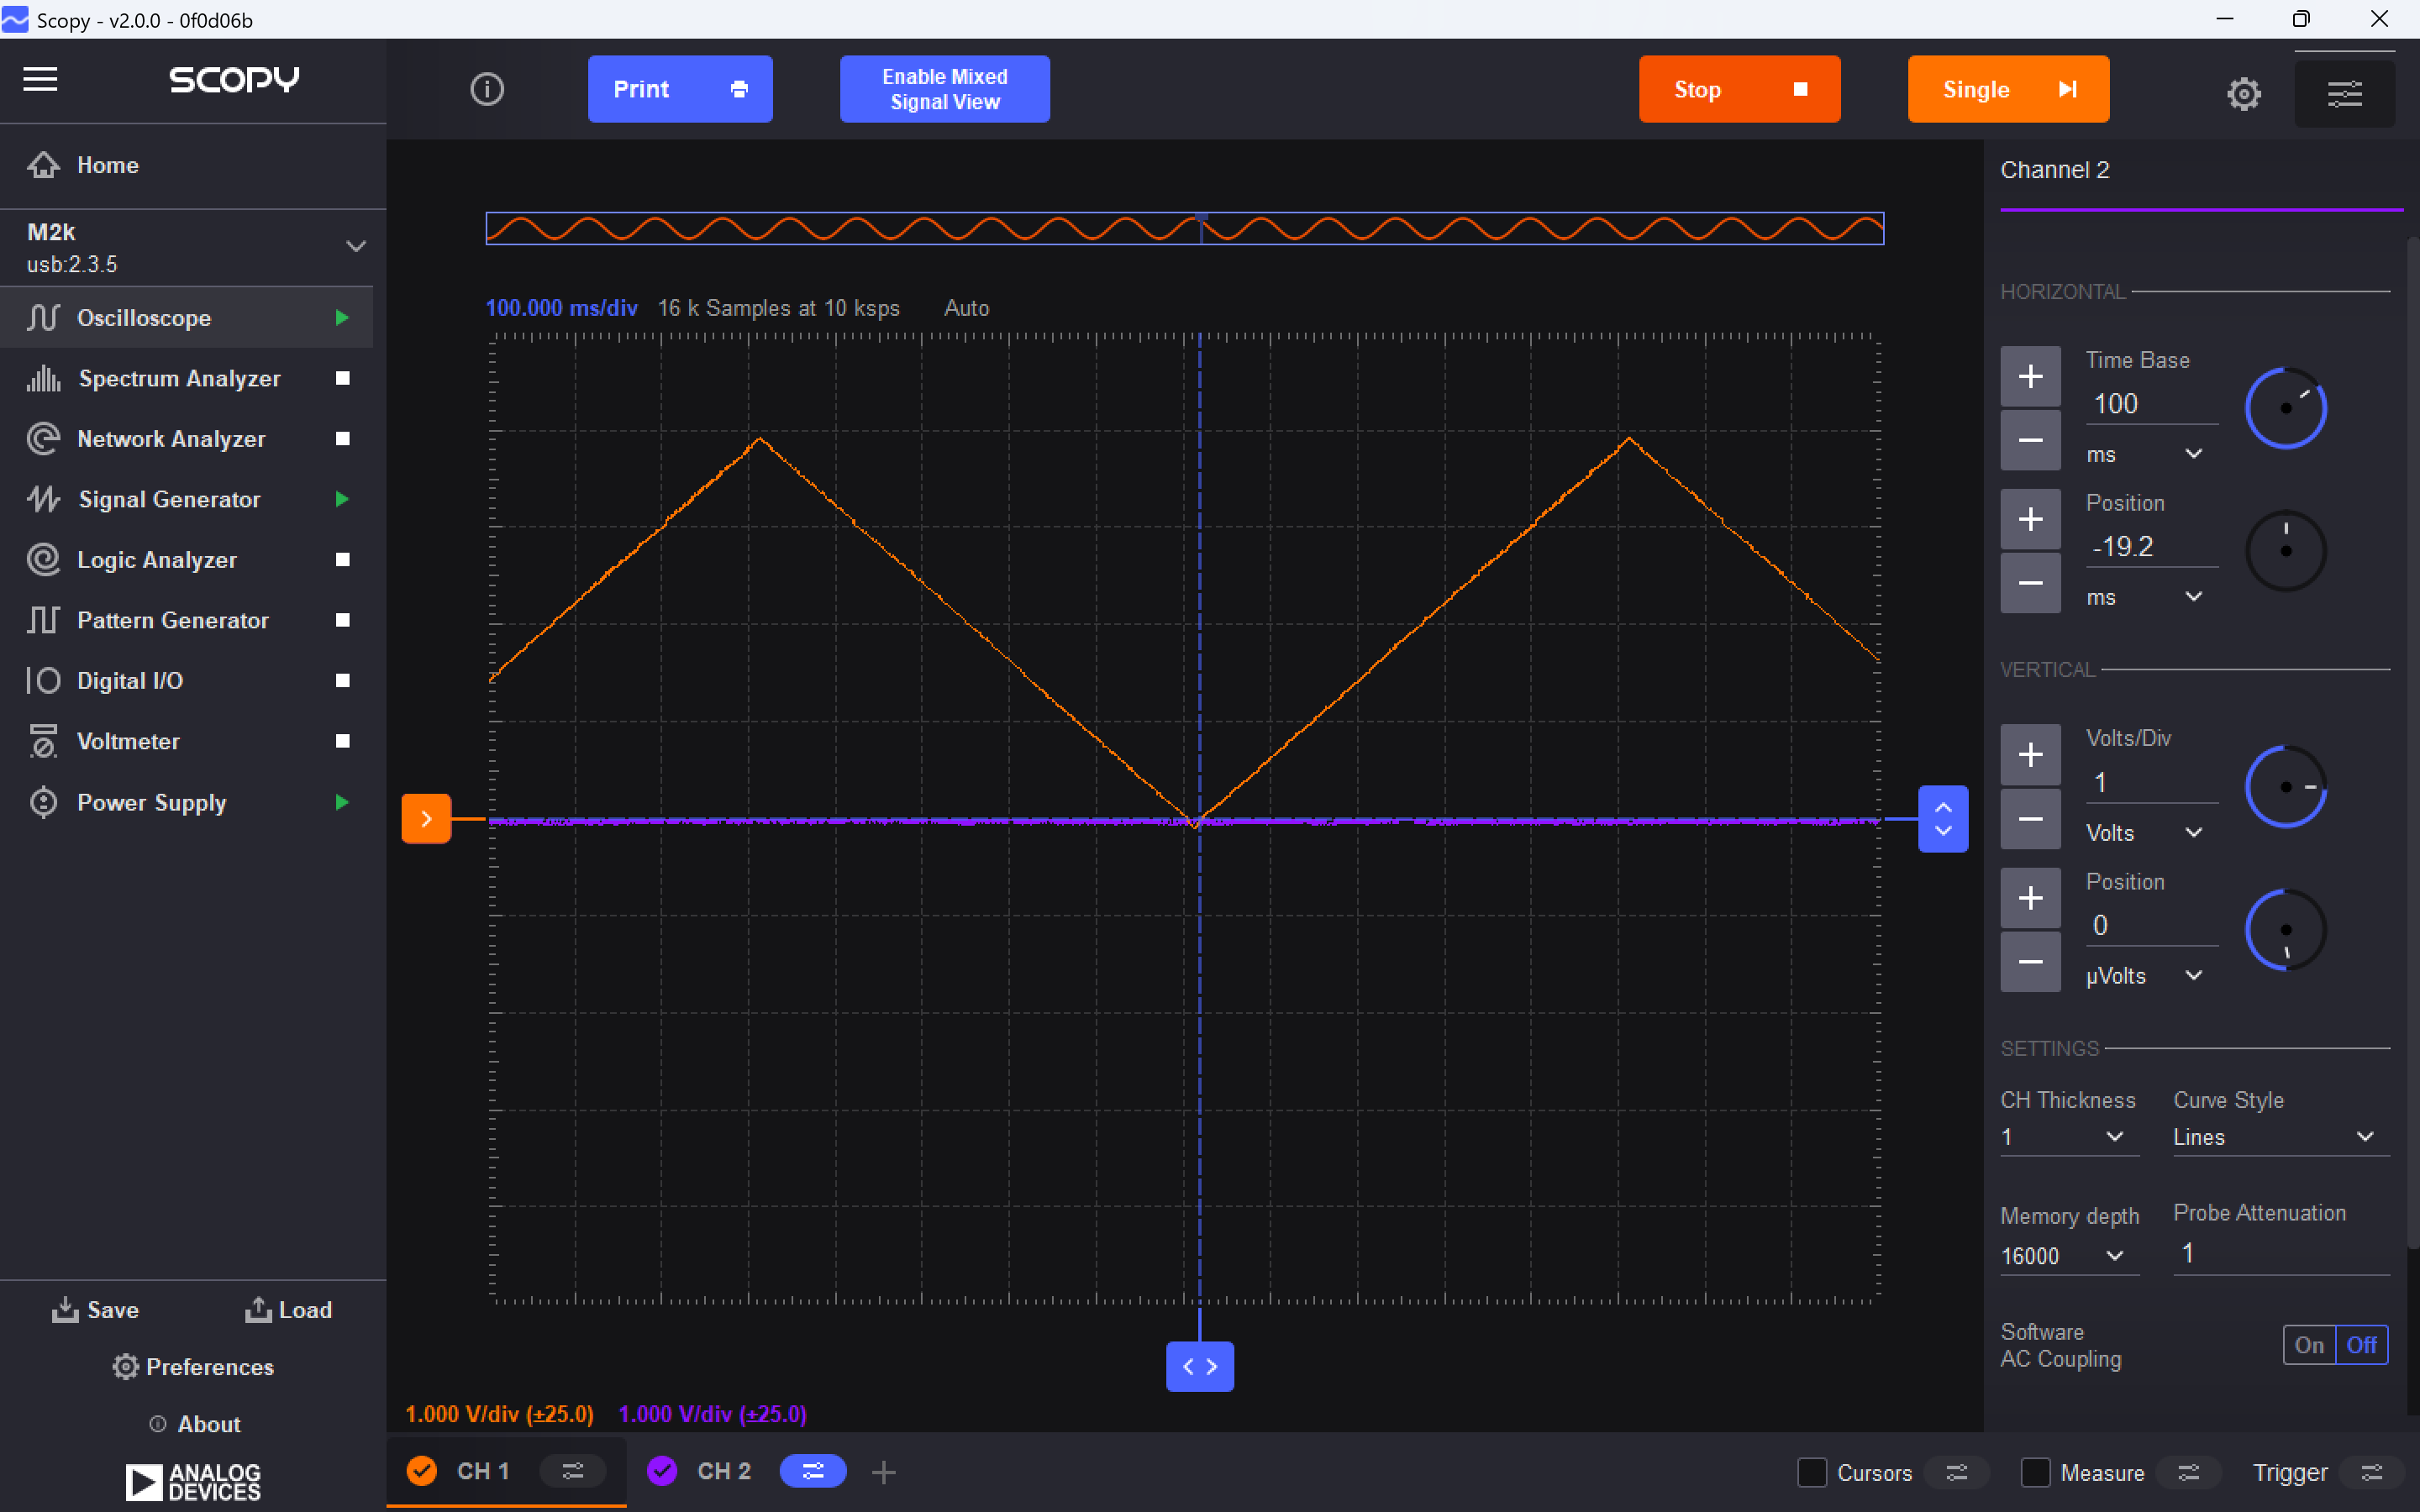
\includegraphics[width=14cm]{04_03}
		      \caption{A Triangle Wave Output}
		      \label{fig:trianglewave}
	      \end{figure}
\end{enumerate}

On all three of the signals, the signal was transformed upwards by the DC Offset
by 2V. This allowed for the signals to stay positive for the most part and have
a minimum of 0V.


\subsection{The Speaker's Amplitude Calculation}
Once the initial setup of the "push-pull" amplifier was completed, the next
steps were to combine the signal generator, the amplifier, and the 8W speaker to
come up with a value which corresponds to an amplitude for a ``Reasonable"
listening volume.
\begin{enumerate}


	\item The circuit in Figure \ref{fig:speakertest} was constructed with the signal
	      generator acting as the input to the operational amplifier.
	      \begin{figure}[H]
		      \centering
		      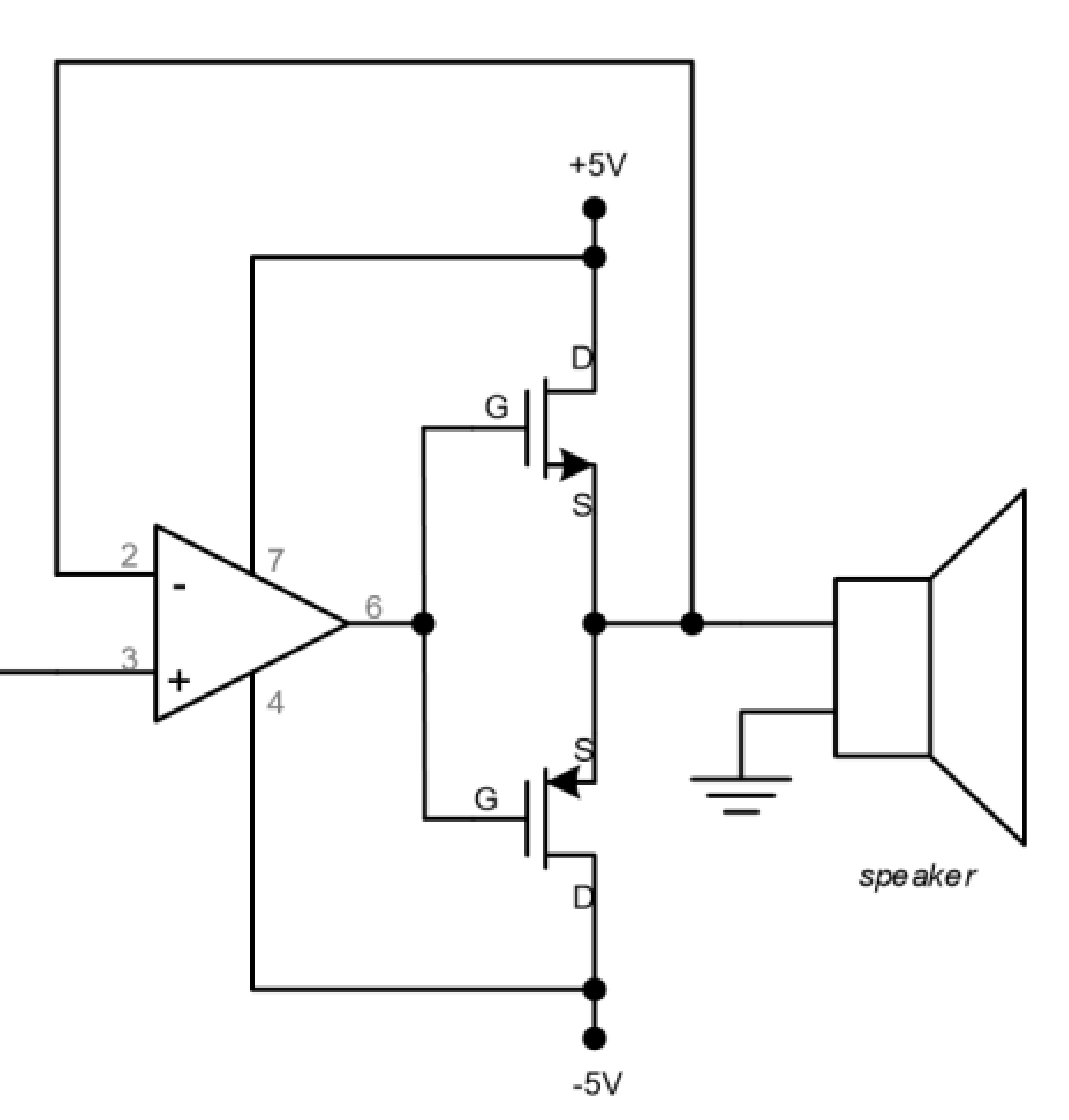
\includegraphics[width=8cm]{04_07}
		      \caption{A Basic Speaker Circuit}
		      \label{fig:speakertest}
	      \end{figure}
	\item A 800Hz sine wave with zero DC offset was generated within Scopy and
	      applied to the circuit.
	\item The amplitude of the signal was adjusted until a tone was produced
	      which correlated to a "reasonable" volume.
	\item This was recorded at 3.3V for my experimental setup.
\end{enumerate}
\subsection{The Electret Microphone}
The next portion of the experiment worked on the input stage of the circuit, the
microphone. The goal here was to find the amplitude of the voltage recorded from
the output of the microphone driven by a 5V circuit shown in Figure
\ref{fig:mictest}

\begin{figure}[H]
	\centering
	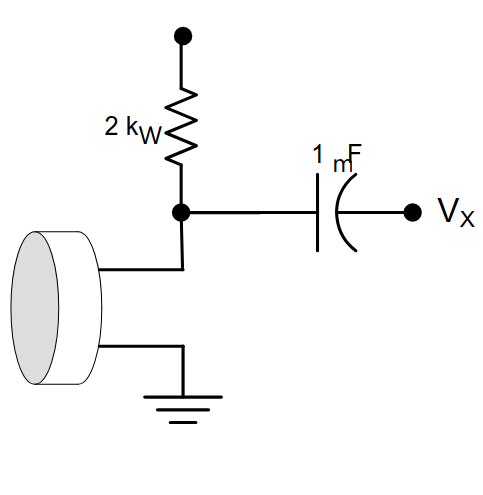
\includegraphics[width=8cm]{04_08}
	\caption{A Microphone Circuit}
	\label{fig:mictest}
\end{figure}
\begin{enumerate}
	\item The circuit was constructed.
	\item The Oscope was connected to the output and dialed in to display the
	      output waveform of the microphone.
	\item Several passes were made with a vocal signal produced 4 inches away
	      from the microphone.
	\item Average peak-to-peak amplitude was recorded at 9mV.
\end{enumerate}
\subsection{An Amplifier Circuit}
As a precursor to the first design project, a theoretical amplifier circuit was
designed in schematic form utilizing the sensitivities recorded in the past
parts.

\begin{enumerate}
	\item The Speaker Sensitivity was \(3.3V\) and the Microphone sensitivity was
	      \(9.9mV\) This means that an amplifier capable increasing the signal by
	      a factor of \(~368\) was necessary.
	\item In order to not saturate the operational amplifier, stages were
	      designed such that they did not exceed 100, and cascaded.
	\item Use of resistors were chosen to not exceed \(1M\Omega\) and be
	      greater than \(1K\Omega\) and standard 5\% tolerance.
	\item The outcome was the first stage utilizing a ratio of 10, and the
	      second stage utilizing a ratio of 36.
	      \[
		      V_{out} = (\frac{-R_B}{R_A})(\frac{-R_D}{R_C})
	      \]
	      When substituted:
	      \[
		      V_{out} =
		      (\frac{-100K\Omega}{10K\Omega})(\frac{-270K\Omega}{7.5K\Omega})
	      \]

	\item The Circuit is shown in Figure \ref{fig:amp}
	      \begin{figure}[H]
		      \centering
		      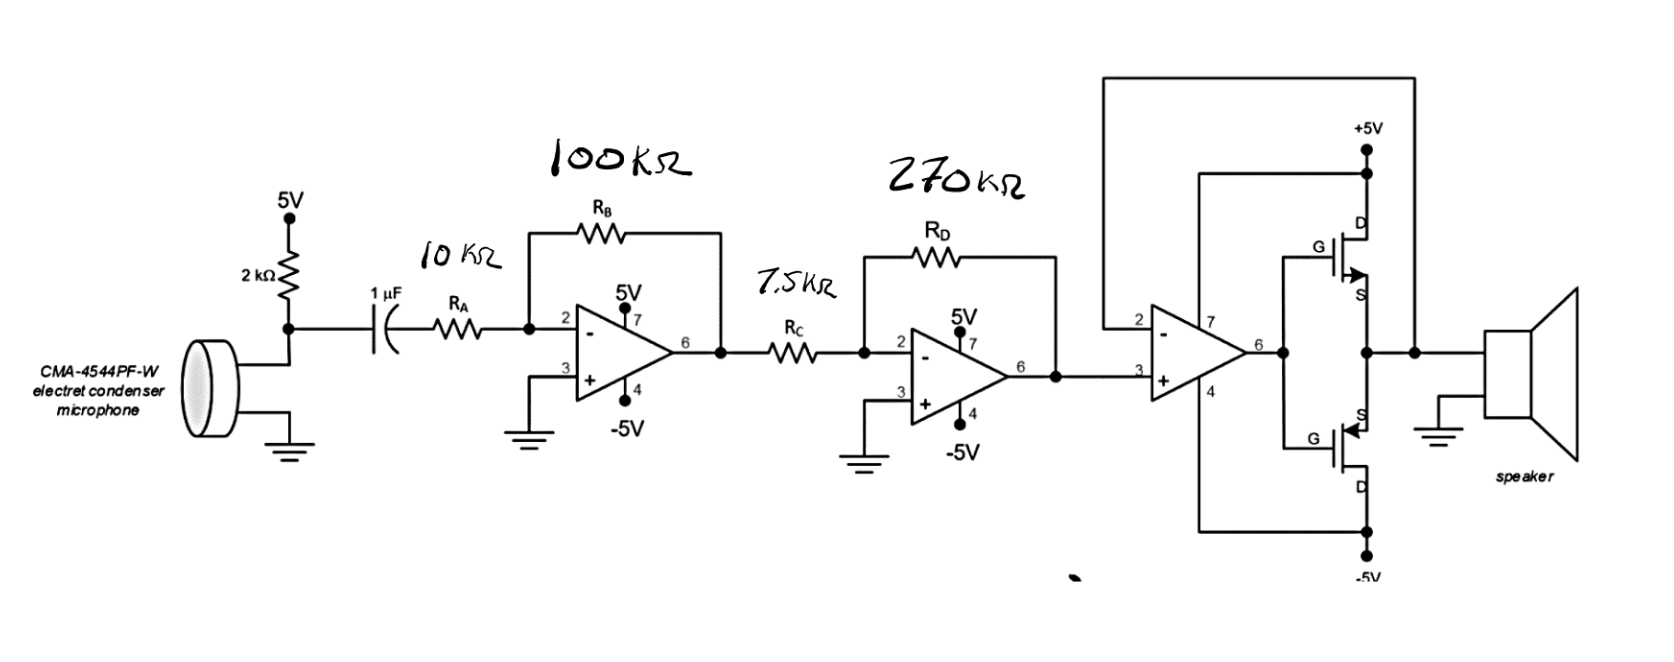
\includegraphics[width=16cm]{04_09}
		      \caption{Amplifier Circuit with Resistor Values}
		      \label{fig:amp}
	      \end{figure}
\end{enumerate}

\subsection{Combining Signals}
The last portion of the experiment combined portions of the previous experiment
and this ones, with a summing amplifier built in hardware. The inputs this time
however are two separate signals from the signal generator.
\begin{enumerate}
	\item The circuit shown in Figure \ref{fig:sumamp} is implemented in hardware.
	      \begin{figure}[H]
		      \centering
		      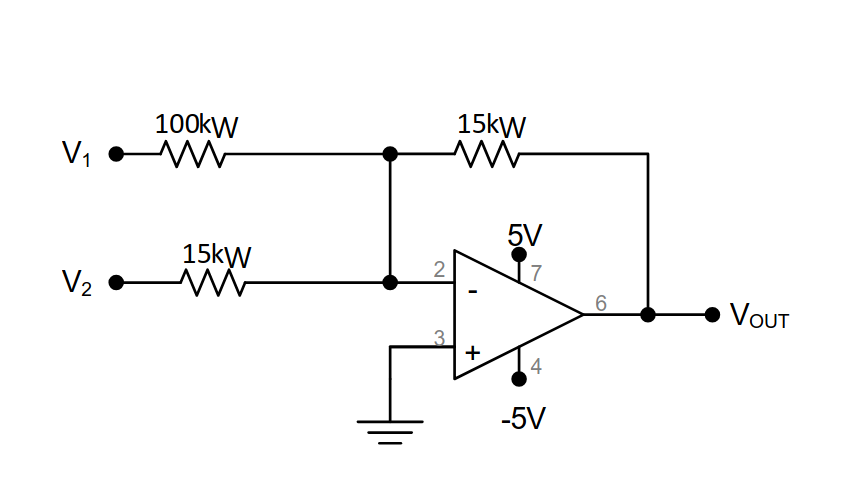
\includegraphics[width=8cm]{04_10}
		      \caption{Summing Amplifier Circuit}
		      \label{fig:sumamp}
	      \end{figure}
	\item The two different signal generator inputs are affixed to the circuit
	      at \(V_1\) and \(V_2\) respectively.
	\item Within Scopy, a Sine Wave of 15kHz and 2V peak-to-peak is generated
	      for the first signal.
	\item A square wave with frequency of 2 kHz and amplitude of 2V
	      peak-to-peak is generated for the second input signal.
	\item The signal is read from Scopy utilizing the oscilloscope function.
	      This signal is displayed in Figure \ref{fig:concat}

	      \begin{figure}[H]
		      \centering
		      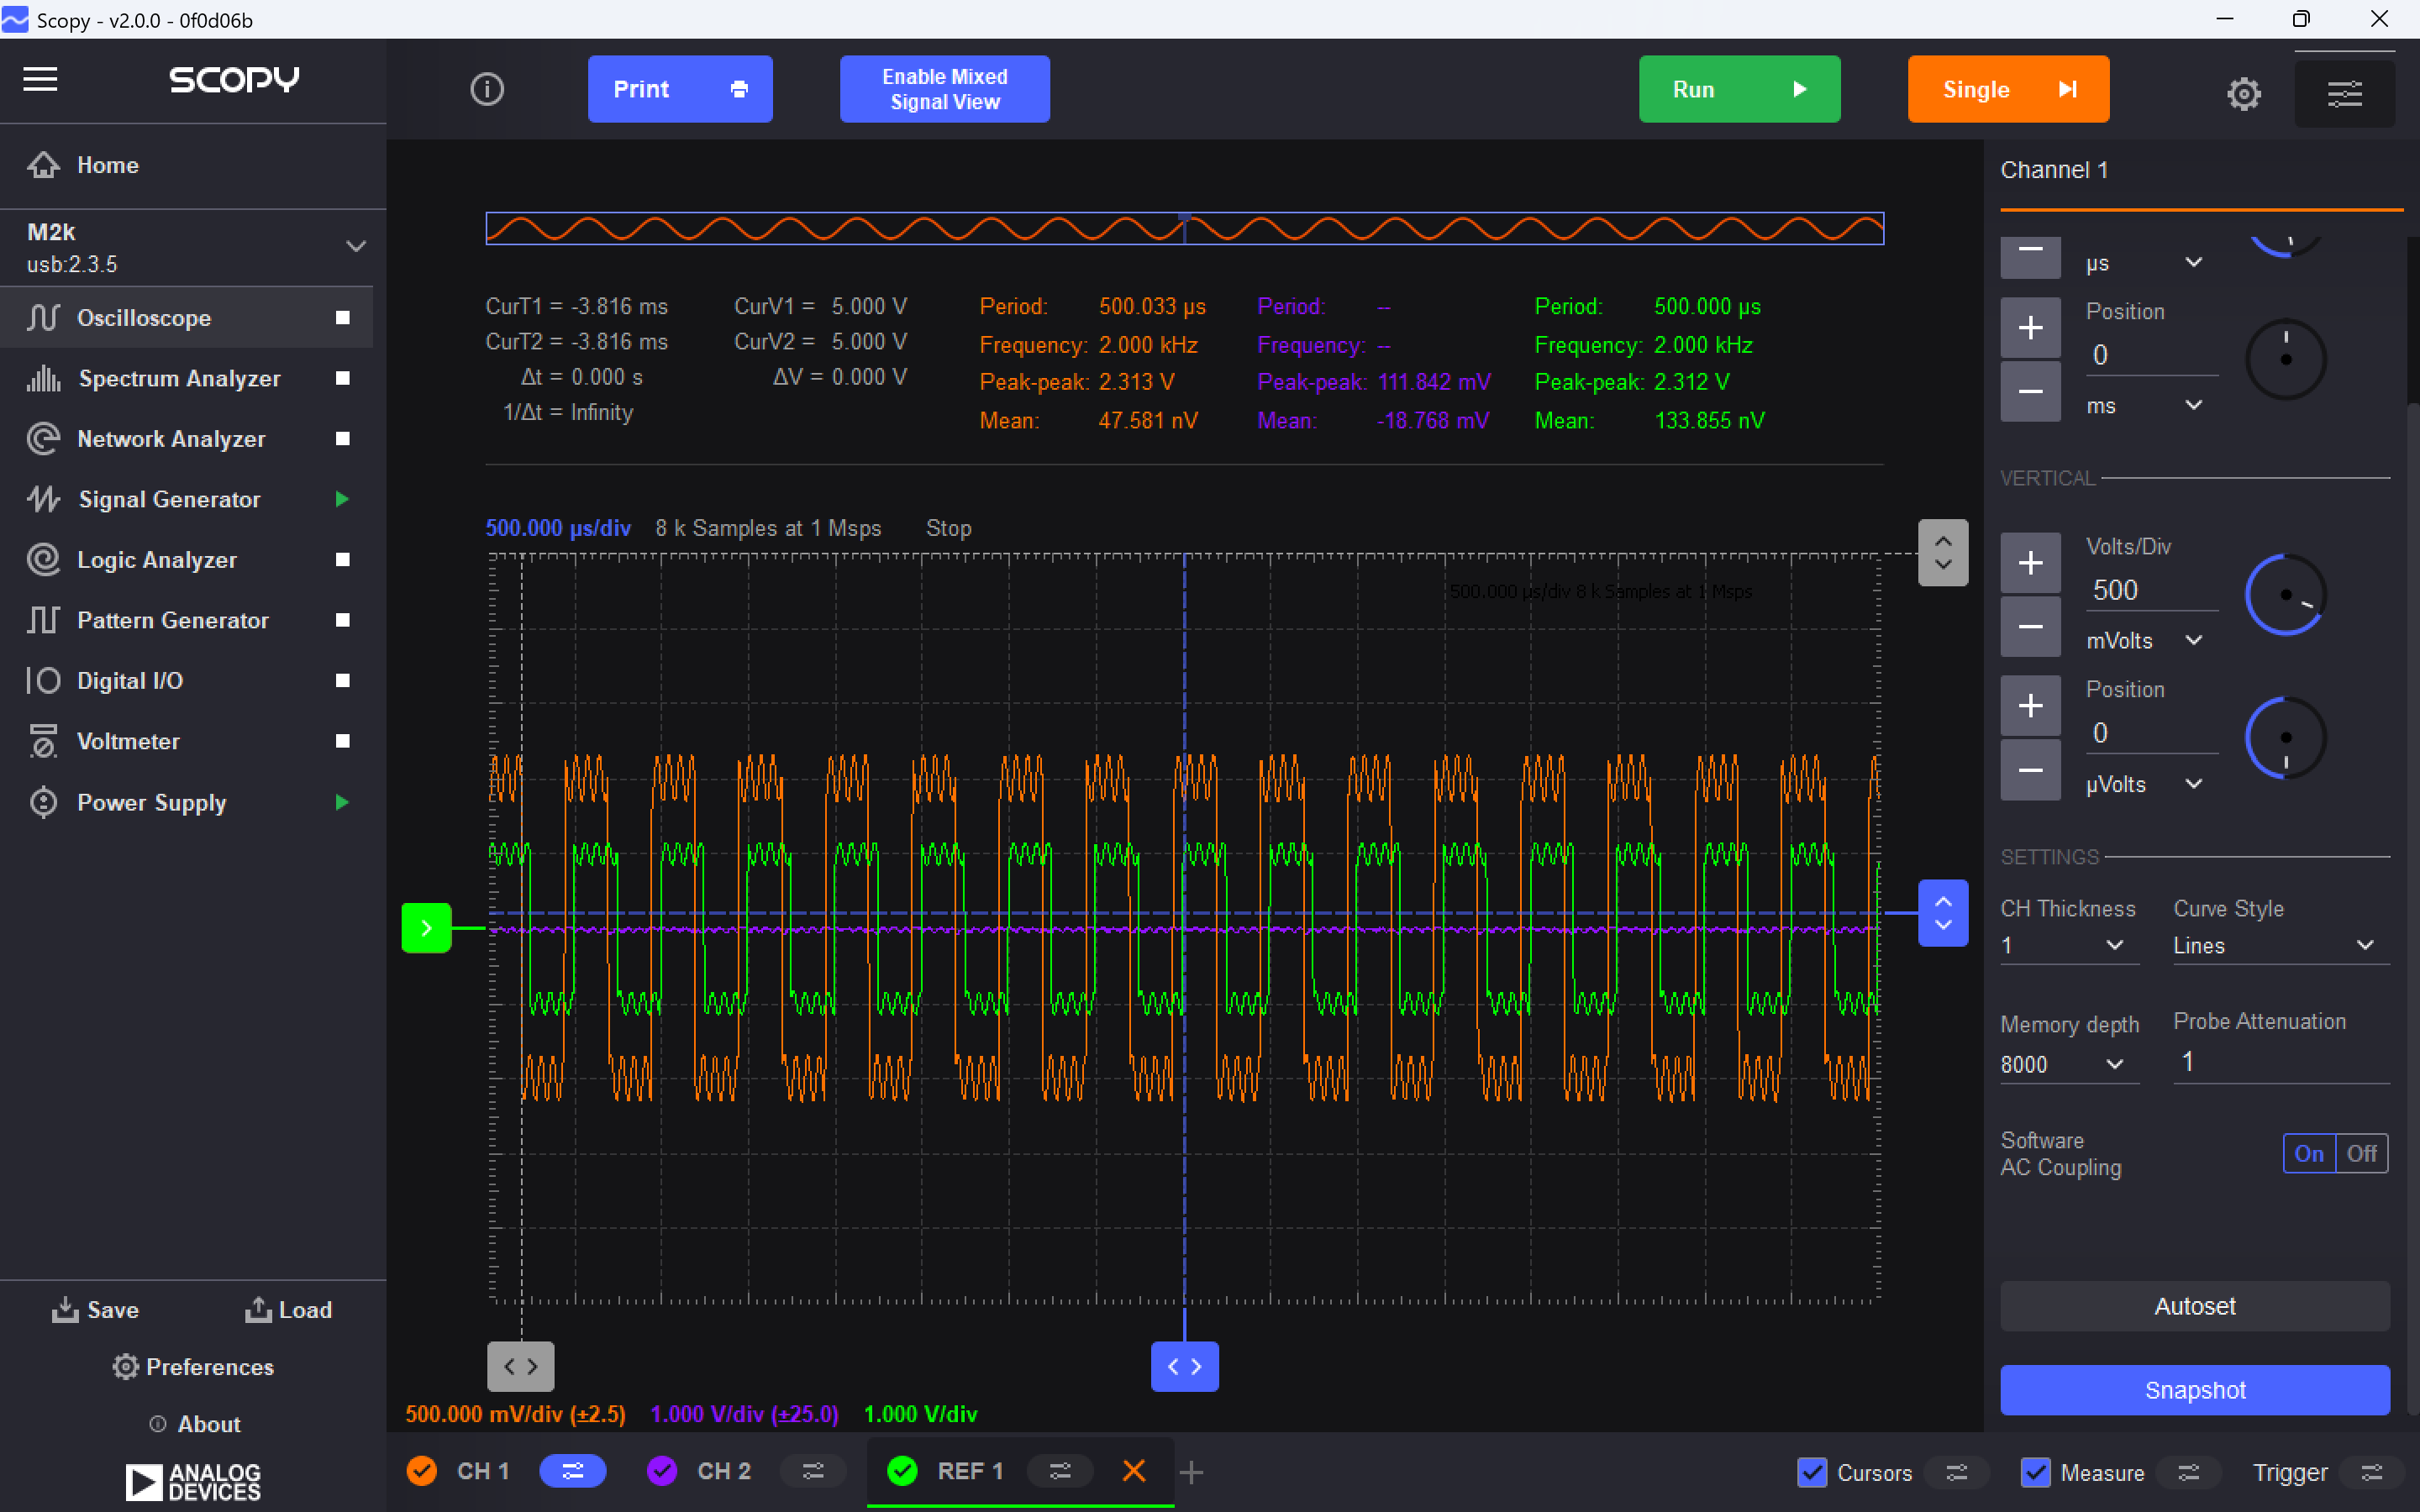
\includegraphics[width=14cm]{04_06}
		      \caption{A Combined Signal}
		      \label{fig:concat}
	      \end{figure}
\end{enumerate}

\section{Results and Discussion}
\subsection{The Signal Generator and Oscilloscope}
Utilizing these new tools provided a new challenge in learning how to not only
connect the equipment correctly to monitor signals, but also in utilizing the
scope to lock in on a variety of alternating signals.

The sine wave was easily able to be locked into with minimal setting change. The
Scopy software provides a way to zoom in horizontally and vertically, known as
the Time Base and the Volts/Div settings. These settings effectively change the
windowing mode within the software and allow for very small signals to be
analyzed.

Understanding the use of waveform/optical physics equations such as the
derivation of period is key for being able to use the oscope correctly. Recall
that Period, \(T\) is calculated by the formula:
\[
	f = \frac{1}{T}
\]
Which show the direct correlation between frequency and period. This insight
provided a huge benefit to find and clean up the signals that were observed in
this portion of the experiment.
\subsection{Testing the Speaker}
Due to electronic components being manufactured over a wide range of tolerances,
the output amplitude of the signal generator had to be found and calculated in
the first step of the design of this circuit.

The sine wave input at 800Hz produced an audible tone from the speaker which was
getting its input from the push pull amplification stage. This served as an
ideal current source which drove the speaker. Because speakers have an internal
impedance to them, a wide variety of input signals need to overcome this. The
amplification stage here acted as that driver.

The input amplitude that was deemed to be "reasonable" was calculated at 3.3V
for my circuit.
\subsection{Testing the Microphone}
This portion of the experiment introduced more experimental ambiguity as
different microphones have different responses. The tricky part of this was to
dial in the scope to be able to accurately trigger, or freeze, on an input
waveform which signified the theoretical input to the eventual amplifier
circuit.

As this was done in a noisy environment, several attempts and passes were made
and an average of 9.9mV was recorded as a solid sensitivity for the electret
microphone. Learning how to use the Scopy software to calculate the peak-to-peak
amplitude and the triggering commands was challenging, but offered reward in
intuition and understanding of the actual microphone sensitivity itself.

The microphone itself is a somewhat complex circuit as it requires its own 5V
power supply alongside a drain resistor and a capacitor which have not been
introduced yet as part of the course. Ultimately, the capacitor acts as a filter
which blocks DC noise input in effect.
\subsection{Preliminary Design}
This section was straightforward as two inverting amplifier stages are
cascaded by design to achieve the desired circuit characteristics while existing
within constraints.

The two stages were chosen such that the first stage does not take too much of
the burden, relying on a ratio of 10 to implement a tenfold amplification. The
subsequent stage then ups the ante by being a ratio of 36. This turns out to fit
nicely within the constraints of the resistors and the stages. However, this
experiment only delved in the conceptual design of the circuit and not actually
implementing it in hardware. Going back to last weeks experiment, the inverting
amplifiers are the most easy to calculate gain for as they are simply a function
of the ratio of the negative feedback loop and input. With this in mind, two
cascaded inverting amplifiers make the output the correct orientation again in
regards to polarity, so this works quite nicely.

\subsection{A Combined Signal}
The last portion of the experiment hints at the potential use cases of the
oscilloscope in a production or test environment. With two different shaped
signals being input into a summing amplifier, an interesting output waveform is
displayed which show the concatenation of two different shaped signals with
different frequencies (15kHz and 2kHz).

Recalling the experimental work in the previous lab, the use of a summing
amplifier results in an output that combines the inputs into a single one. The
operational amplifier was originally used as a chip to perform mathematical
operations, and coming from the purely mechanical world of the early 20th
century to the beginning of the digital era (not quite yet though) this offers
insight into what made sense to engineers of the era.

With two different shaped signals input into the operational amplifier, a really
strange output is observed which shows a square sine wave... or is it a sine
square wave? Nevertheless, the interpretation is such that the overlying shape
of the signal is a combined form of the two inputs, which is expected behavior
of the circuit. The screen grab shows an additional waveform, which is in the
green color that is not to be confused with the triggered waveform in orange.
This is simply leftover of the measure function of Scopy, which was used to tune
in on the waveform within the viewing window.

\section{Conclusion}

Audio amplifiers are used everywhere from playing music to
making announcements on a nuclear submarine to keep the crew on the same page
and are a vital step in understanding electric circuitry.

This experiment successfully introduces the signal generator and oscilloscope
into our arsenal of test equipment for further enrichening knowledge of
electrical circuits. By gradually introducing the use of these tools, the
expectation to design a circuit that can amplify an acoustic signal is prepared
for. Without diving too deep into things like silicon doping and the gating of
the MOSFETs, the use of the operational amplifier is elaborated upon and shown
in a practical way as well as the mystical ideal current source built.
The utilization of Scopy alongside the ADALM2000 as a signal generator and
oscilloscope offer a novel way to analyze these signals without the need for an
extensive lab setup. The introduction of different wave shapes and frequencies
allows for further insight into audio generation.

\end{document}
% vim: set ft=tex tw=80 ts=2 sts=2 sw=2 noet spell:
